% Derived from PGF's diamond, star, and trapezium border-anchor algorithms.
\documentclass[border=2pt]{standalone}
\usepackage{tikz}
\usetikzlibrary{arrows.meta,shapes.geometric}

\begin{document}
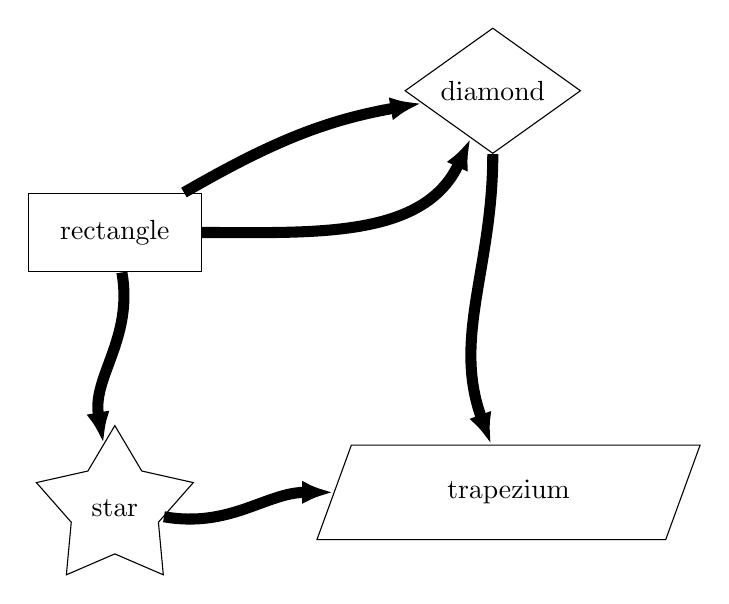
\begin{tikzpicture}[x=1cm,y=1cm]
  \node[draw,rectangle,minimum width=2.2cm,minimum height=1cm] (rect) at (0,0) {rectangle};
  \node[draw,diamond,aspect=1.4,minimum width=2cm,minimum height=1.5cm] (diamond) at (4.8,1.8) {diamond};
  \node[draw,star,star points=5,star point ratio=1.8,minimum size=1.8cm] (star) at (0,-3.5) {star};
  \node[draw,trapezium,trapezium left angle=70,trapezium right angle=110,minimum width=2.2cm,minimum height=1.2cm] (trap) at (5,-3.3) {trapezium};

  \draw[-{Latex[length=4mm,width=3mm]},line width=4pt] (rect) to[out=30,in=190] (diamond);
  \draw[{Latex[length=4mm,width=3mm]}-,line width=4pt] (diamond) to[out=245,in=0] (rect);
  \draw[-{Latex[length=4mm,width=3mm]},line width=4pt] (rect) to[out=-80,in=100] (star);
  \draw[-{Latex[length=4mm,width=3mm]},line width=4pt] (diamond) to[out=-90,in=110] (trap);
  \draw[{Latex[length=4mm,width=3mm]}-,line width=4pt] (trap) to[out=180,in=-10] (star);
\end{tikzpicture}
\end{document}
